\section{Systematic uncertainties}
\label{sec:systematics}
The sources of systematic uncertainties are summarized as
follows:
\begin{itemize}
\item Background-related systematic uncertainties: background parametrization.
\item Signal-related systematics uncertainties: W/Z-tagging efficiency, Jet Energy Scale(JES), Jet Energy Resolution(JER), luminosity.
\end{itemize}

\subsection{Background shape parametrization}
\label{sec:background}

We model the shape of the QCD background in the dijet spectrum 
using a simple parametrization which has been sucessfully deployed in
previous searches in the dijet mass spectrum~\cite{cmsdijet}.
The background model is given in Eq.~(\ref{eqParam}):
\begin{equation}
\frac{{\rm d}N}{{\rm d}m} = 
\frac{P_{0} (1 - m/\sqrt{s})^{P_{1}}}{(m/\sqrt{s})^{P_{2}
}} .
\label{eqParam}
\end{equation}
\noindent where $m$ denotes the dijet mass and $\sqrt{s}$ the pp center of mass energy.
$P_0$ acts as a normalization parameter for the probability
density function, and $P_1$, $P_2$ describe its shape.
It was checked by a Fisher F-test that no additional parameter is not needed to discribe the distributions.

Figure \ref{fig:singleVtagBG} and Figure \ref{fig:doubleVtagBG} show the dijet mass spectra from
single and double $\PW/\cPZ$-tagged data fitted to Eq.~(\ref{eqParam}) and the bottom panes show corresponding pull
distributions, demonstrating the agreement between the background-only
probability density function and the data.

No sizeable deviation from the background-only hypothesis is seen,
exclusion limits are set on the product of cross section, acceptance, and branching fraction for
the five considered final states: qW, qZ, WW, WZ, and ZZ.

\begin{figure}[th!b]
\begin{center}
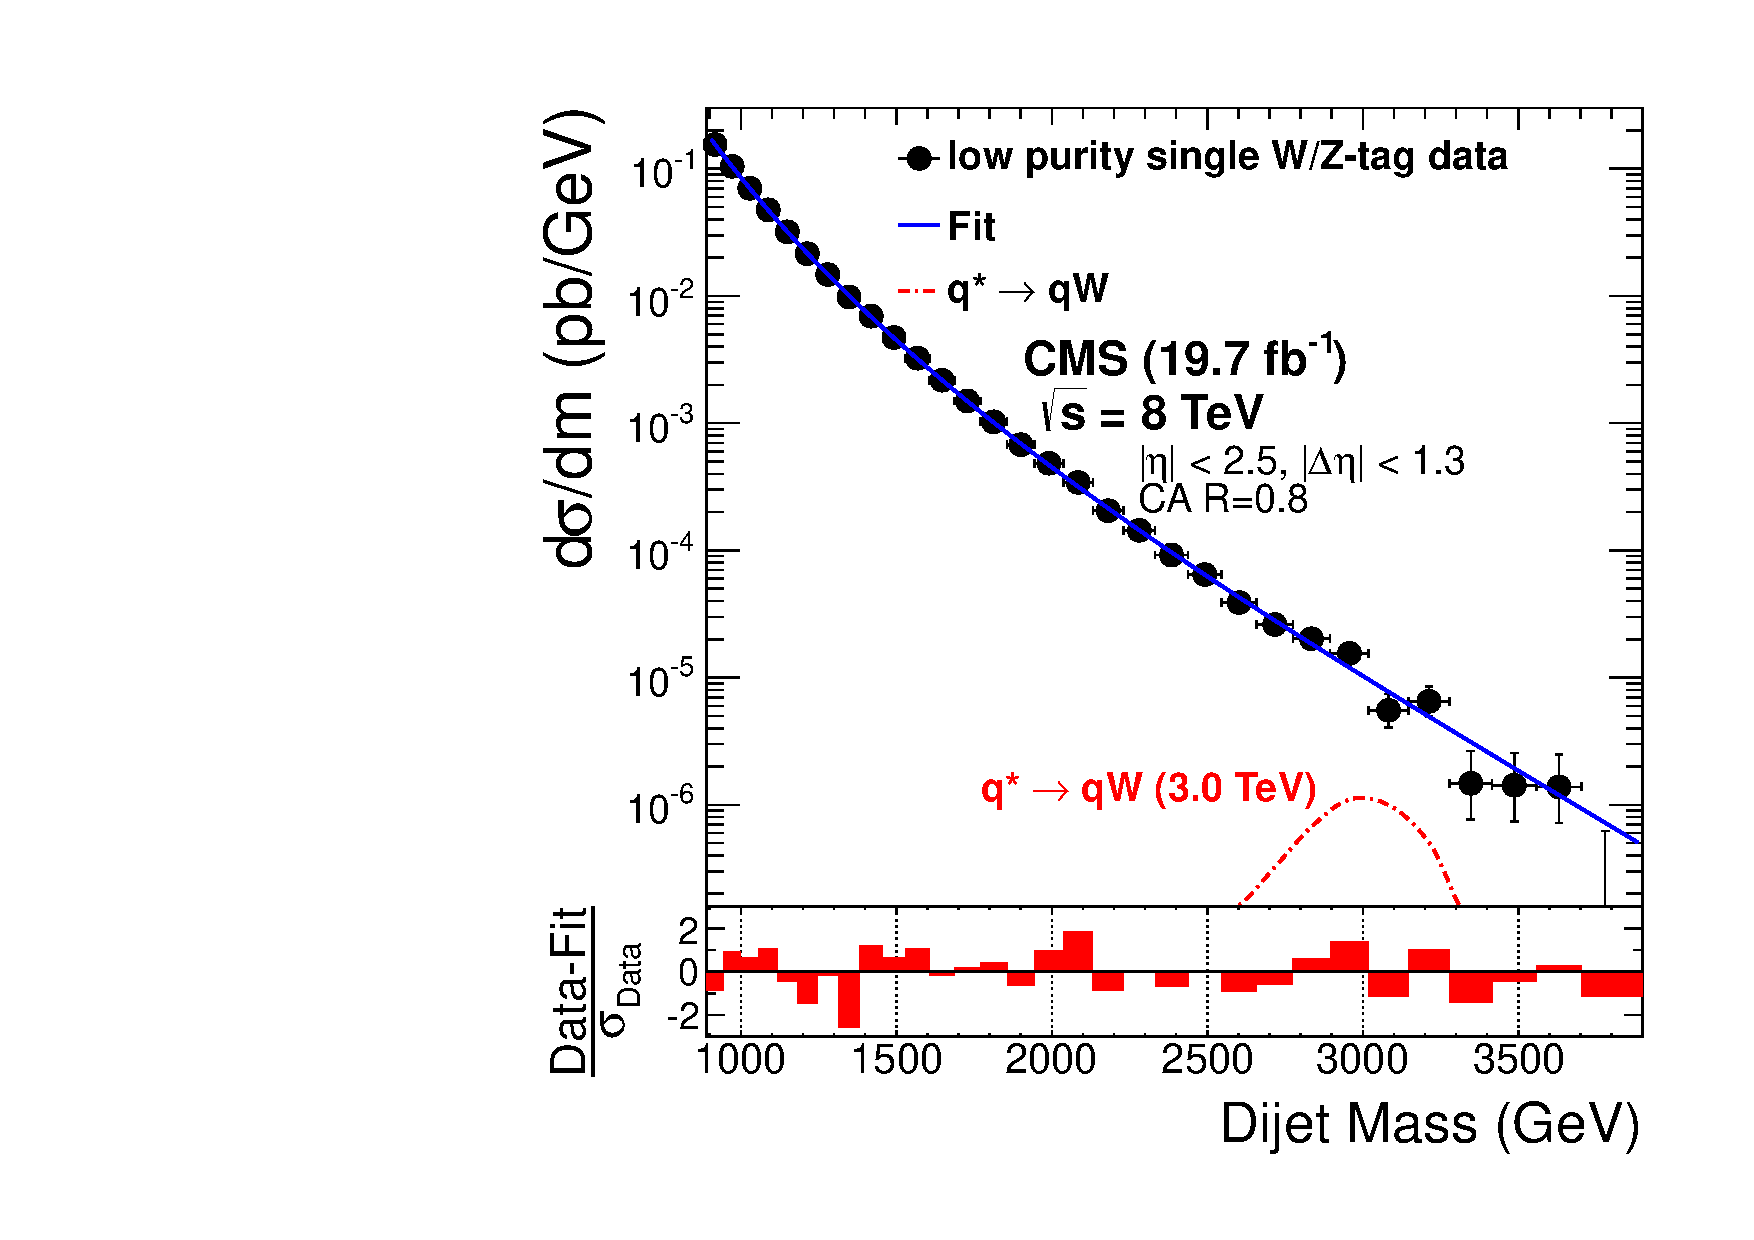
\includegraphics[width=0.49\textwidth]{figs/MediumPuriqVFitAndPull.pdf}
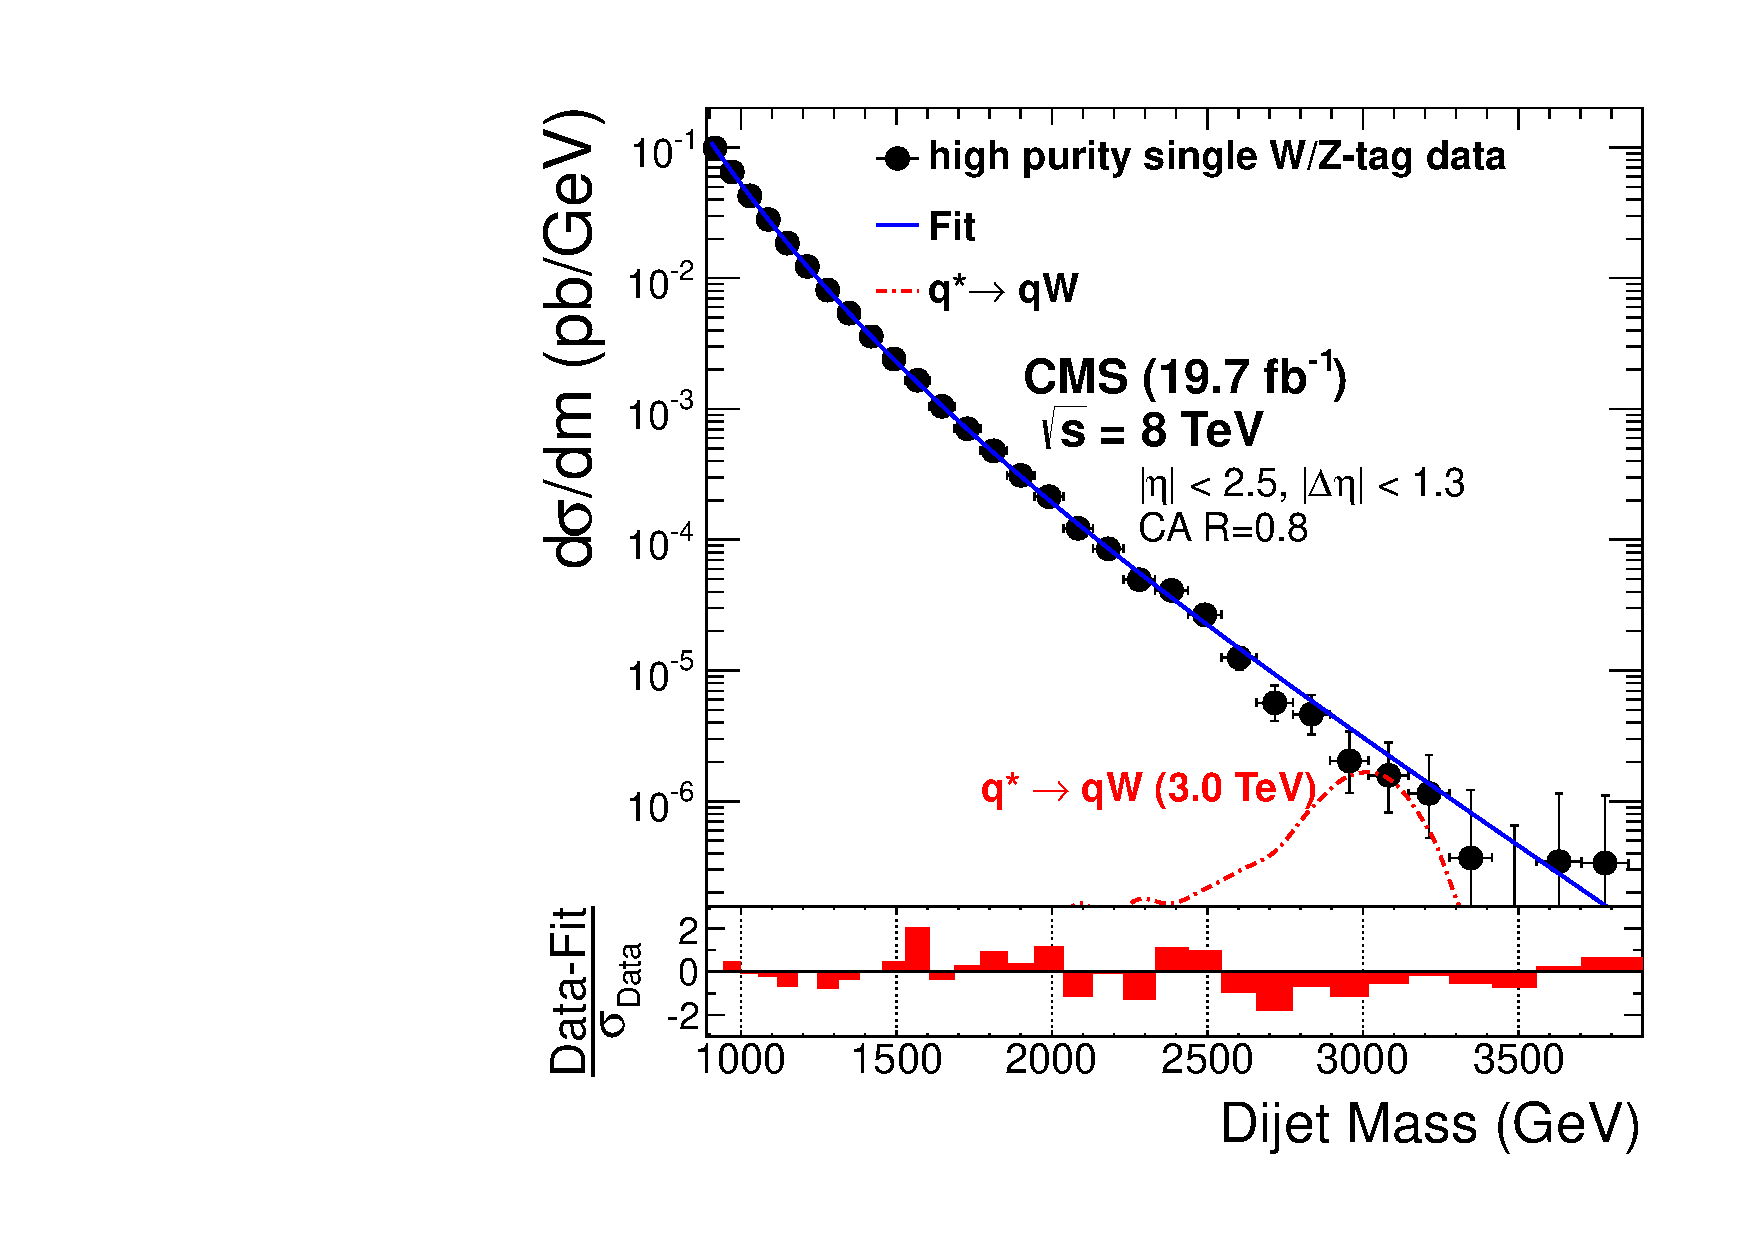
\includegraphics[width=0.49\textwidth]{figs/HighPuriqVFitAndPull.pdf}
\end{center}
\caption{The medium purity (\cmsLeft) and high purity (\cmsRight) single $\PW/\cPZ$-tagged $m_{jj}$
  distributions (points) in data fitted with the QCD background parametrization (solid
  curve).  Signal shape distribution for $\cPq^* \to \cPq\PW$
   with its corresponding cross section is also shown.  Bottom panes:
  the corresponding pull distributions ($\frac{\text{Data}-\text{Fit}}{\sigma_{\text{Data}}}$).  }
\label{fig:singleVtagBG}
\end{figure}

\begin{figure}[th!b]
\begin{center}
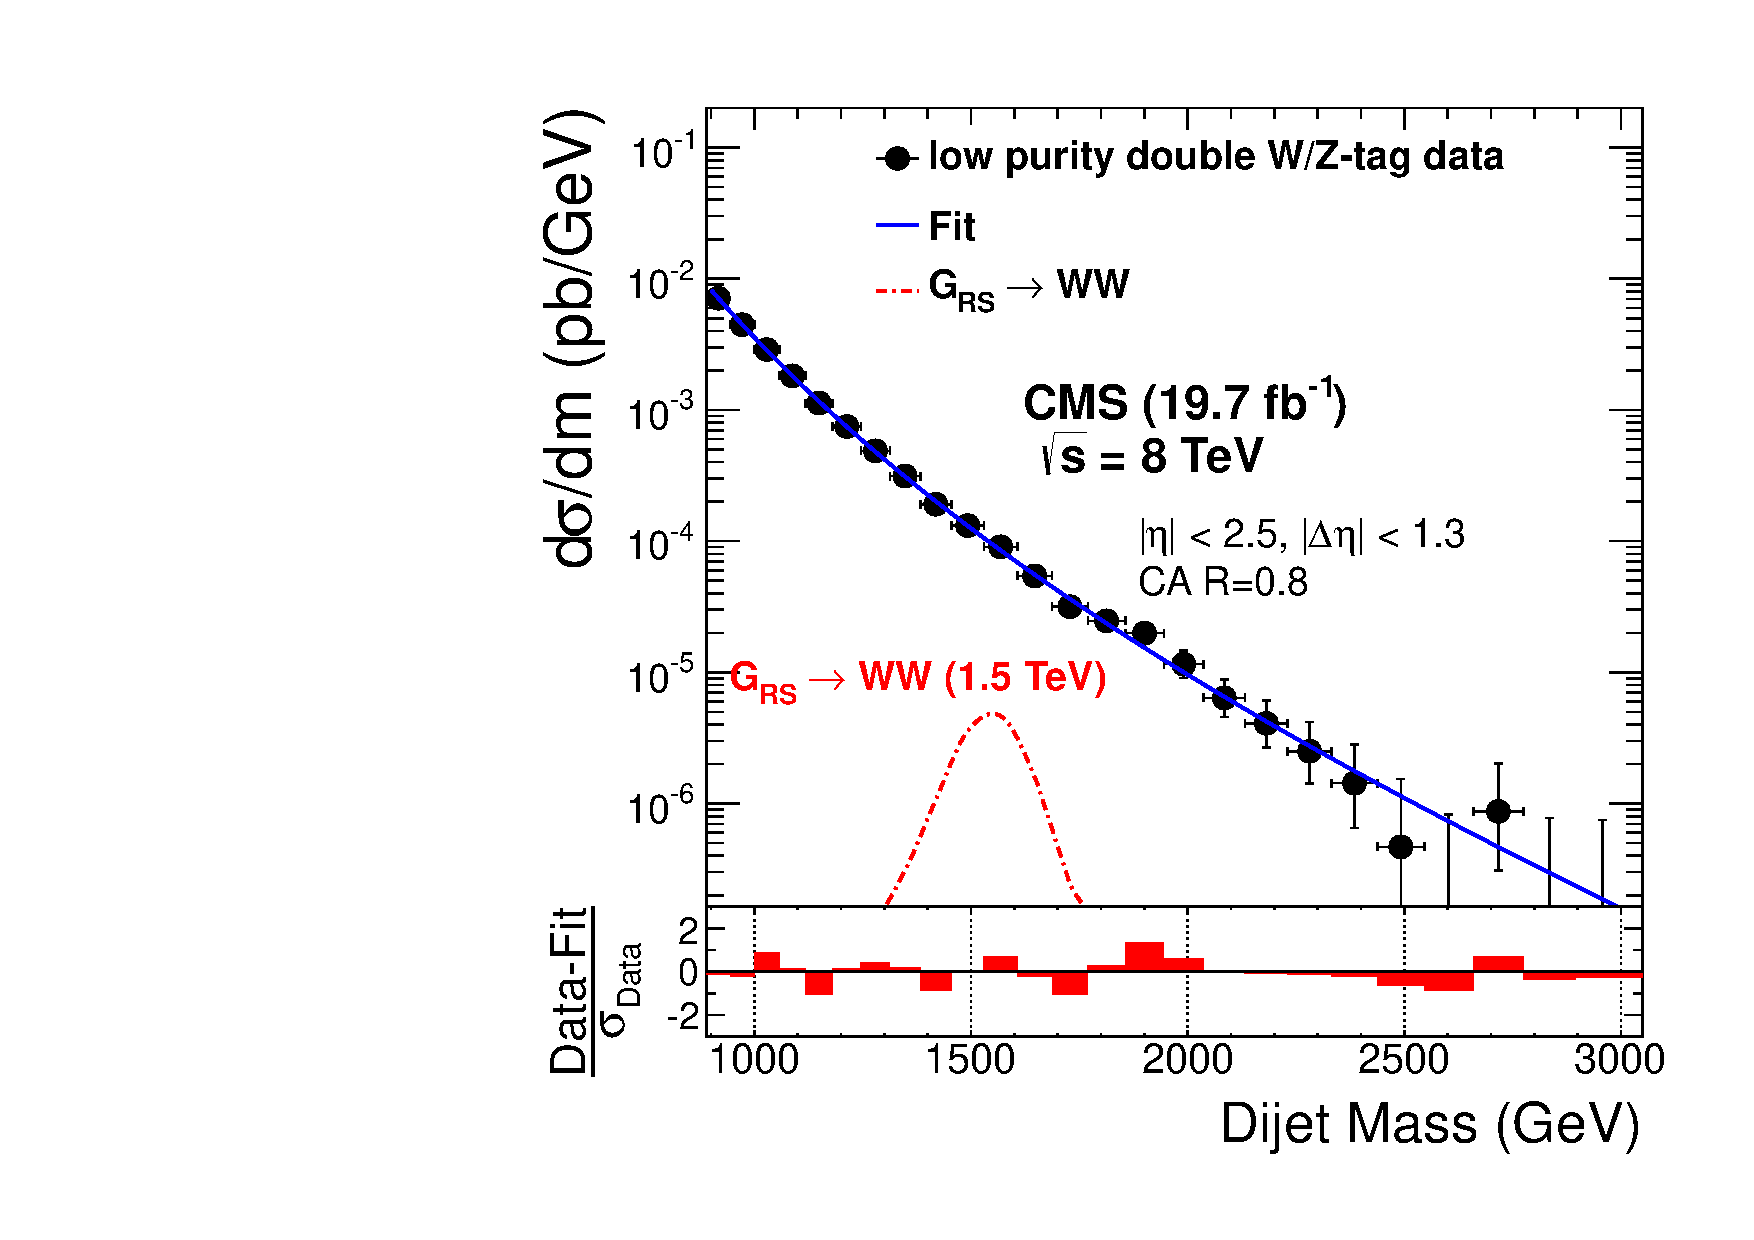
\includegraphics[width=0.49\textwidth]{figs/MediumPuriVVFitAndPull.pdf}
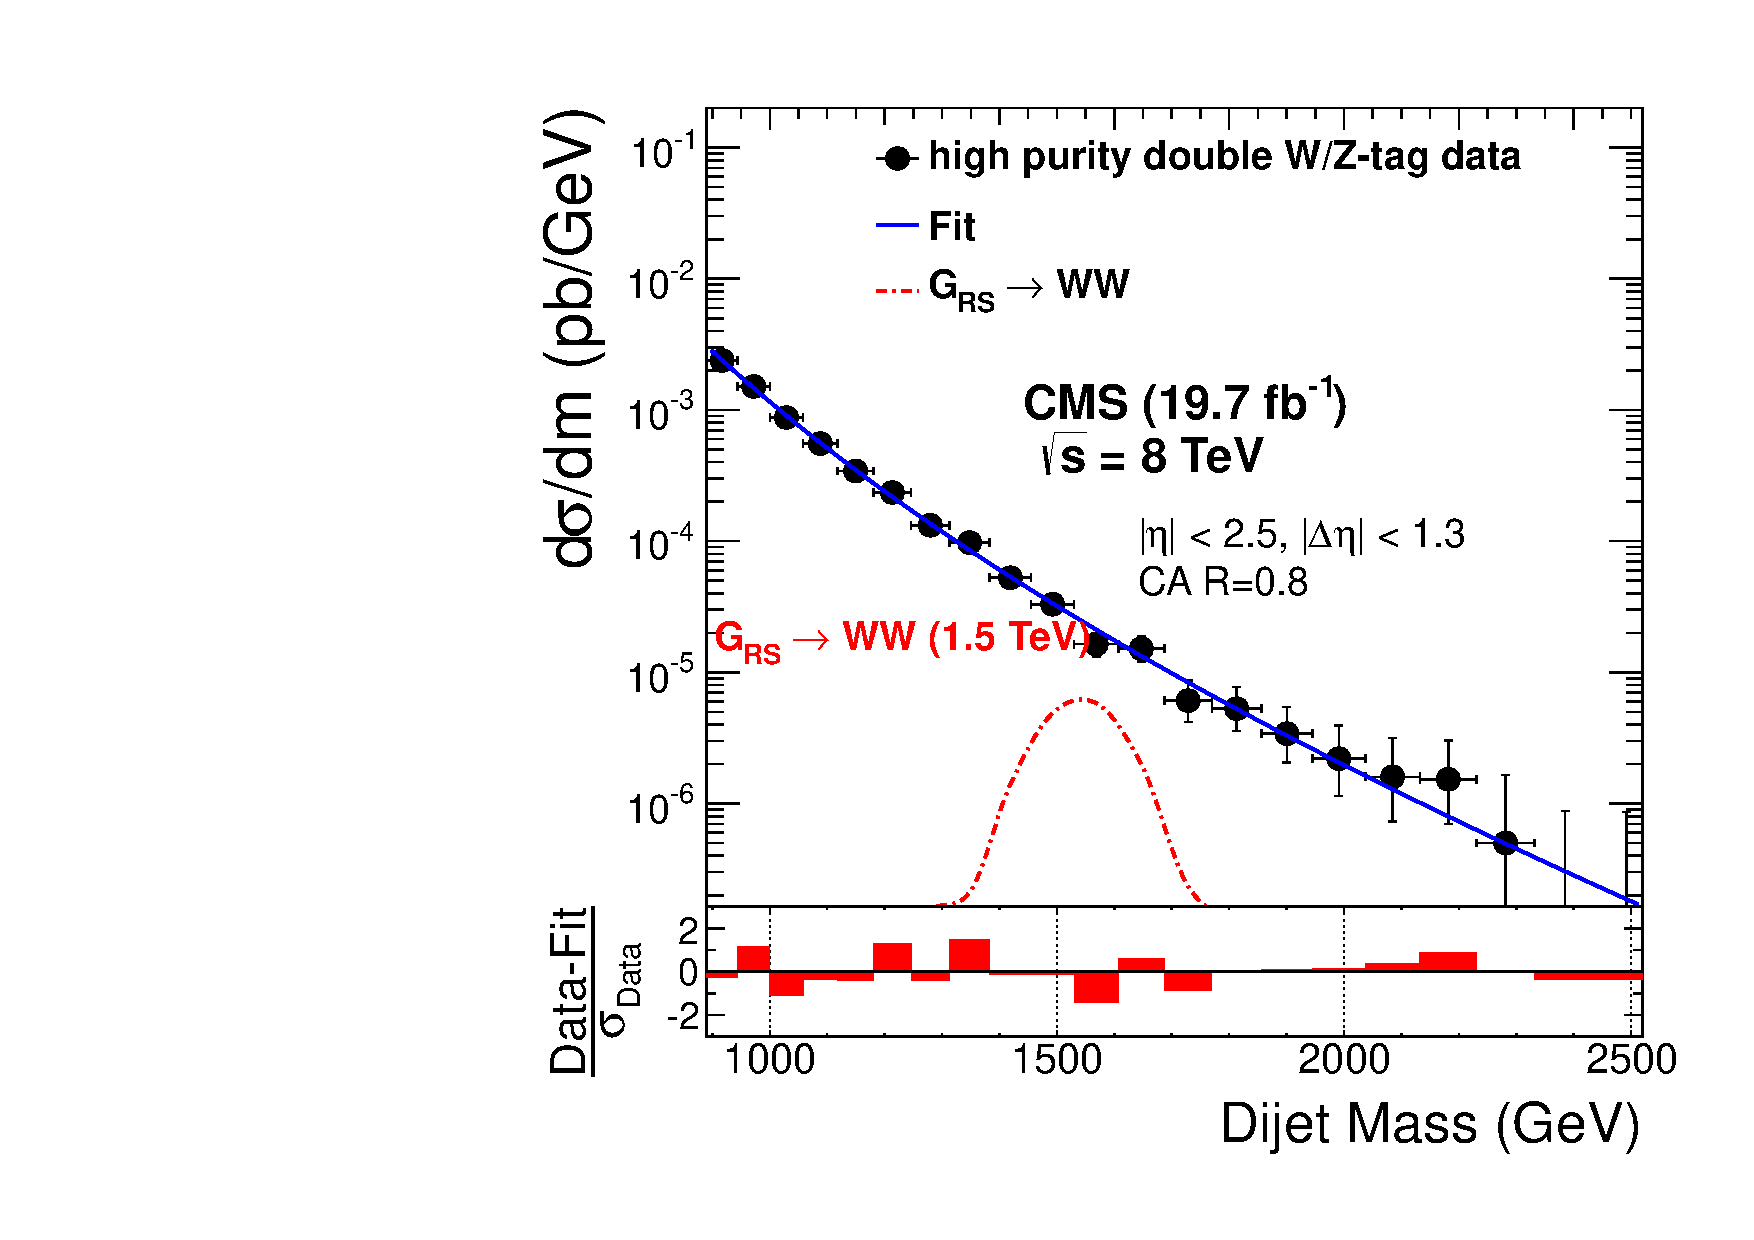
\includegraphics[width=0.49\textwidth]{figs/HighPuriVVFitAndPull.pdf}
\end{center}
\caption{The medium purity (\cmsLeft) and high purity (\cmsRight) double $\PW/\cPZ$-tagged $m_{jj}$
  distributions (points) in data fitted with the QCD background parametrization (solid
  curve).  Signal shape distribution for
  $\GRS \to \PW\PW$ with its corresponding cross section is also shown.  Bottom panes:
  the corresponding pull distributions ($\frac{\text{Data}-\text{Fit}}{\sigma_{\text{Data}}}$).  }
\label{fig:doubleVtagBG}
\end{figure}



\subsection{W/Z-tagging efficiency}
\label{sec:vtageff}

The W/Z-tagging efficiency is determined from the Monte Carlo simulation.
We cross-check the MC modelling of the signal efficiency by measuring the W/Z-tagging efficiency
in semileptonic $\ttbar$ data, and compare it
with the same efficiency obtained using identical procedure from $\ttbar$ Monte Carlo sample generated with MadGraph~\cite{madgraph} and showered with Pythia6 Tune Z2*.
The ratio of the two efficiencies defines a scale factor, which is then applied to
the efficiencies for signals in the dijet data.

We follow the same procedure as described in Ref.~\cite{JME-13-006}.
%The efficiency of the cut on the $\tau_{21}$ variable in the semileptonic $\ttbar$ sample is found to be \mucuteffsemilepdata for data, %and \mucuteffsemilepmc for Monte Carlo.
%The efficiency of the pruned jet mass cut for the data and Monte Carlo are \mcuteffsemilepdata and \mcuteffsemilepmc, respectively.
Combining the efficiencies of the $\tau_{21}$ and jet mass cuts, a data-MC scale factor of  \scalefactorHP
(\scalefactorLP) for the high (low) purity selection for the  W-tagging efficiency is determined.
We assume that the same scale factor applies to \zboson-tagging as well.
The errors on the scale factor are propagated
into the systematic uncertainties on the overal signal efficiency.


%\begin{figure}[htb]
%\centering
%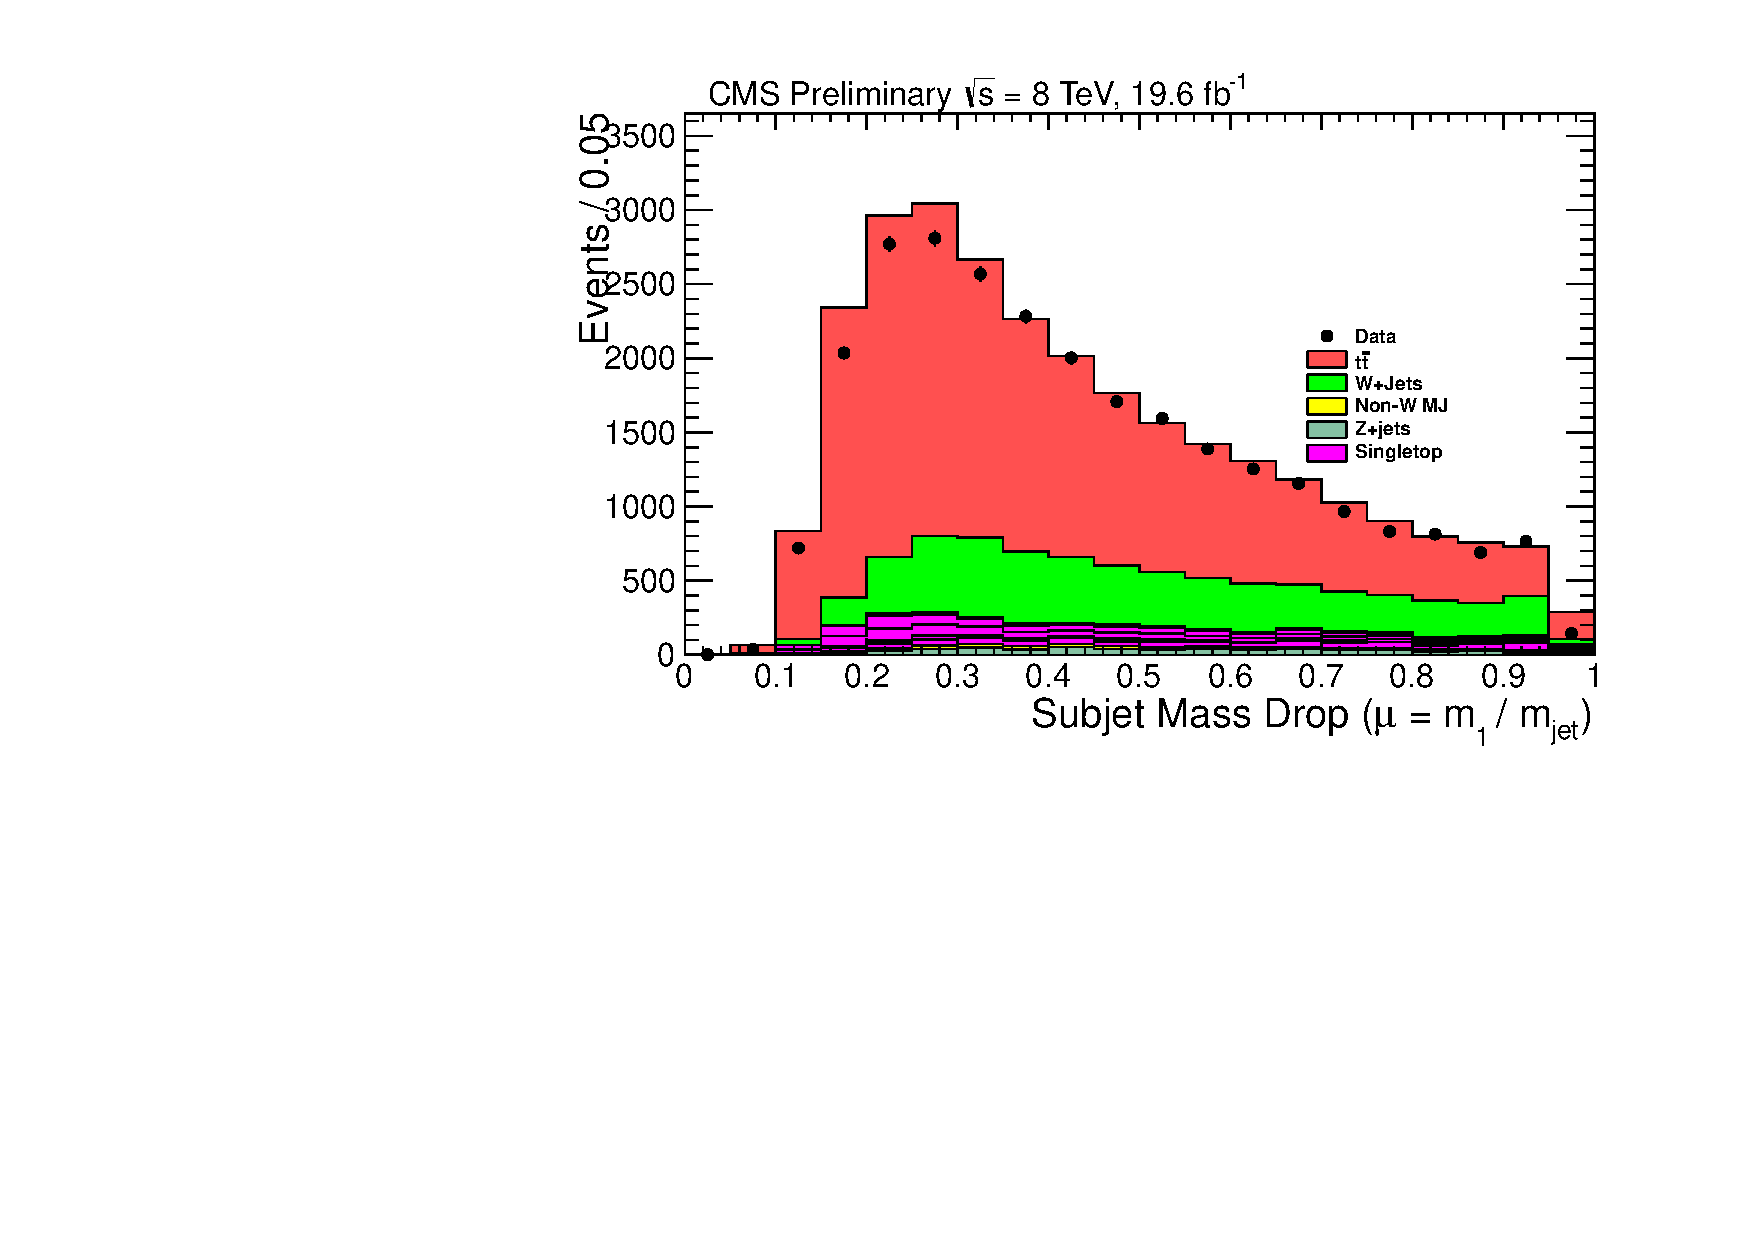
\includegraphics[width=0.95\textwidth]{figs/semiLepMass_muHist}
%\caption{$\tau_{21}$ of the highest mass jet in a semileptonic
%ttbar sample from Ref.~\cite{hadronictop}.}
%\label{figs:muHist_semileptonic}
%\end{figure}

%\begin{figure}[htbp]
%\centering
%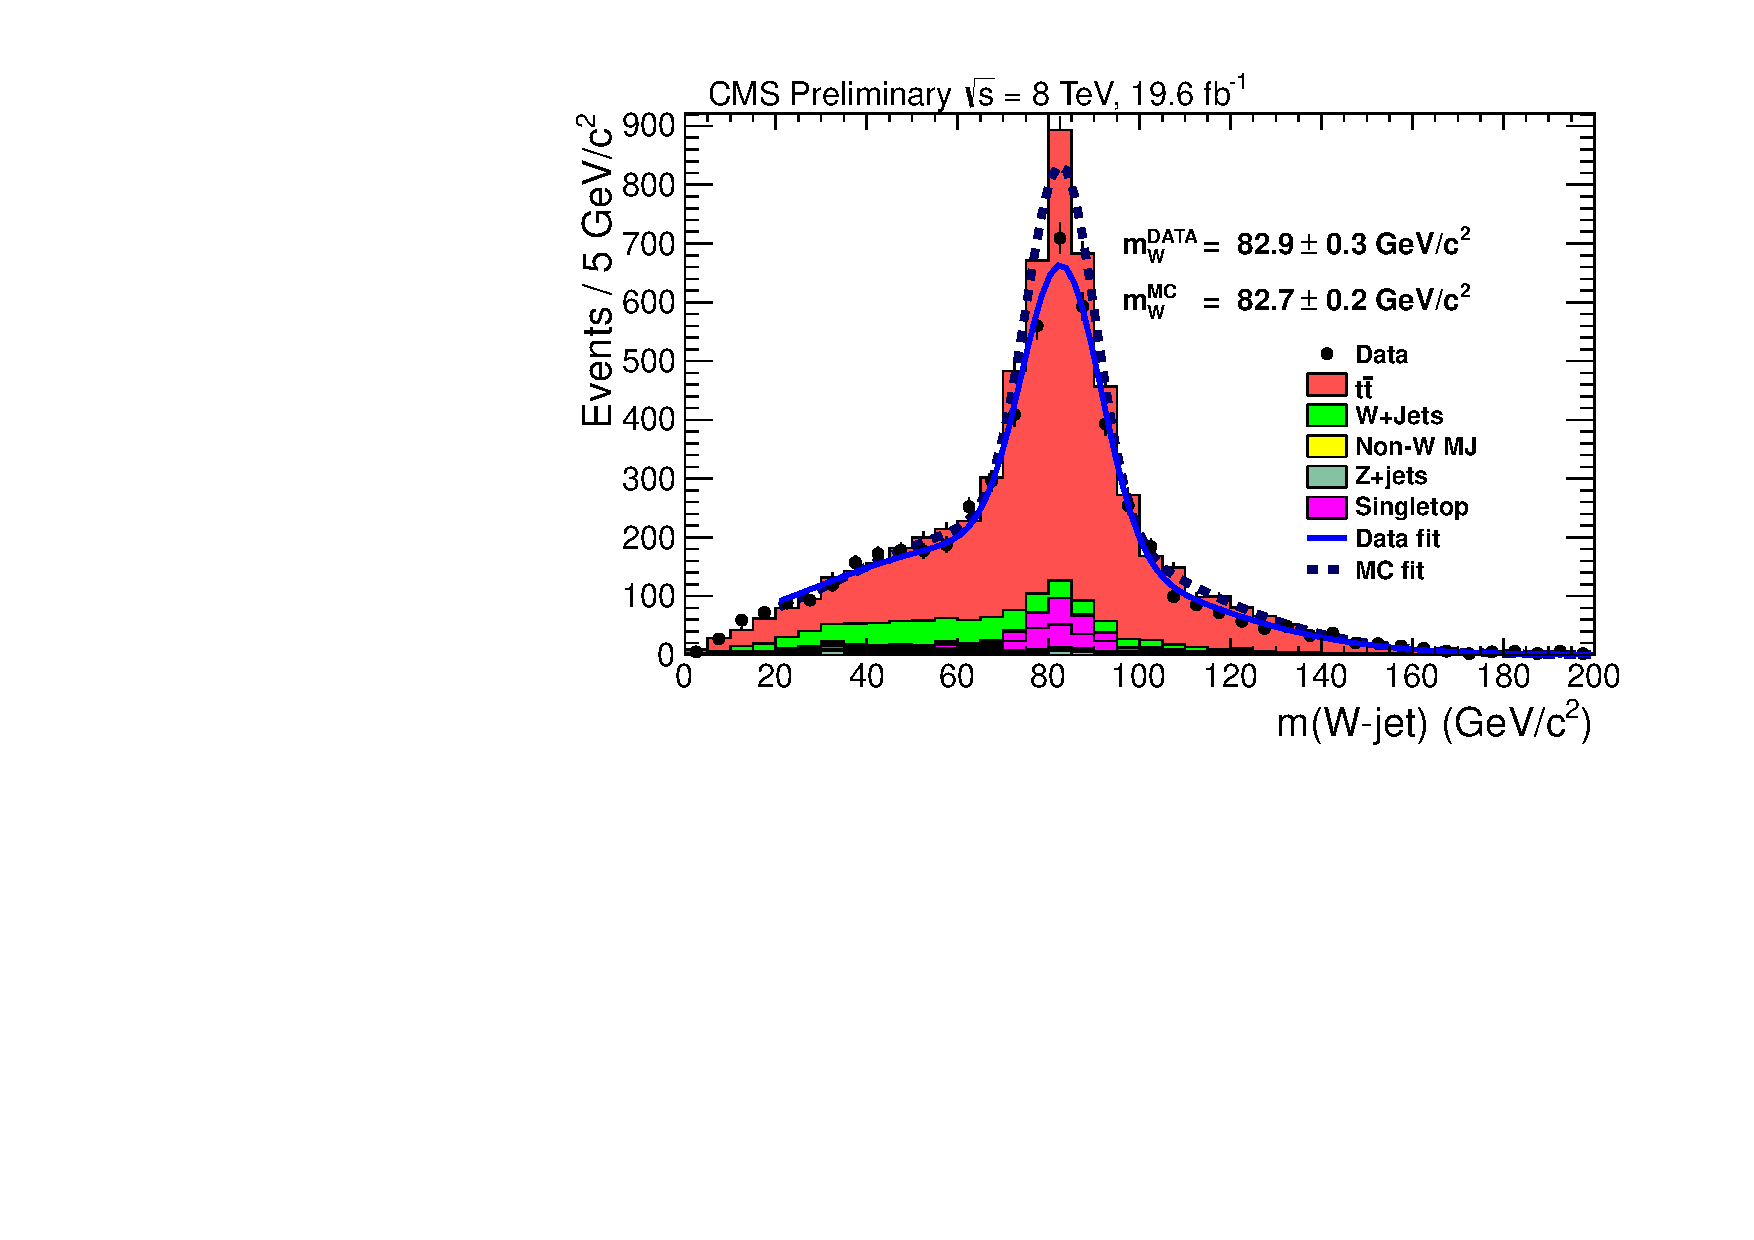
\includegraphics[width=0.95\textwidth]{figs/semiLepMass_mWCand.pdf}
%\caption{Pruned jet mass of the highest mass jet in a semileptonic
%ttbar sample from Ref.~\cite{hadronictop}.}
%\label{figs:mHist_semileptonic}
%\end{figure}


The efficiency error on a single $\PW/\cPZ$-tagging is estimated with
a control sample of semileptonic $t \bar t$ events as described above.
The uncertainties of \scalefactorHPu (\scalefactorLPu) on the scale
factors for high (low) purity tagging include sources from control
sample statistics, pruned jet mass scale and pruned jet mass
resolution.
Since we estimate the scale factor
only in the kinematic regime of the $\ttbar$ sample where the W decay
products merge, but the b-quarks are still reconstructed as separate
jets, we need to rely on the simulation to extrapolate to
higher jet \pt.
Therefore, we estimate how the efficiency varies as a function of
\pt for two different showering and hadronization models using
\GBulk samples generated with {\sc jhugen} and interfaced with
\PYTHIA~6 and \HERWIG{++}.
We find that the differences are within $4\%$ ($12\%$)
for the high (low) purity tagging and therefore smaller than the
statistical uncertainty of the scale factor.
Also, the dijet mass dependence of the $\PW/\cPZ$-tagging efficiency for
background events, shown in Fig.~\ref{fig:singleefficiencies} and Fig.~\ref{fig:doubleefficiencies},
is adequately described by the simulation.
Other systematic errors on the tagging efficiency are small or
negligible.  Because of the rejection of charged particles not
originating from the primary vertex and also the application of
pruning, the pileup dependence on the $\PW/\cPZ$-tagging efficiency
is weak, and the uncertainty of the modeling of the pileup
distribution is less than 3\%.  Modeling of the underlying event,
estimated by switching it off in \PYTHIA~6, impacts the tagging
efficiency by less than 1\%.   These
systematic errors refer to a single $\PW/\cPZ$-tagged jet and are
applied twice for double $\PW/\cPZ$-tagged events.

\subsection{Other uncertainties}

In the jet \PT and $\eta$ regions considered in this analysis, the Jet Energy Scale is known to a precision of 1-2\%~\cite{JME-JINST,Collaboration:2013dp}.
The \PT and $\eta$ dependent uncertainty is propagated to the reconstructed dijet invariant mass, resulting in an uncertainty of 1\% to a good approximation independent of the reconstructed dijet invariant mass.
It is taken into account by shifting the resonance dijet mass in the statistical analysis.
The Jet Energy Resolution(JER) is known to a precision of 10\% and its tails are in agreement between data and MC~\cite{JME-JINST}.
It is taken into account in the statistical analysis by a variation of the resonance width by 10\%.
The luminosity has been measured with an uncertainty of 2.6\%~\cite{LUM-13-001}, and is also taken into account in the statistical analysis.

\clearpage
